% Chapter 1 - Introduction
\chapter{Introduction} % Main chapter title
\label{Chapter1} % For referencing the chapter elsewhere, use \ref{Chapter1} 
%Copied from Thesis Topic Manual
%Introduction
%The introduction should provide the following:
% background to the topic;
% brief review of current knowledge (this is not the literature review – it’s only a high level overview);
% state hypotheses;
% indicate gaps in knowledge, state aims of the thesis and how it fits into the gap;
% an outline of the following chapters.

% The introduction should follow the recommended structure:
% state the general background of the thesis topic and give some background
% provide an overview of the literature related to the thesis topic
% define the terms and scope of the thesis
% outline the current situation
% evaluate the advantages/ disadvantages of existing solutions and identify the knowledge gap
% identify the importance of the proposed research
% state the research problem/ questions
% state the research aims and/or research objectives
% state the hypotheses
% outline the experiment methodology
% outline the structure of the thesis
%----------------------------------------------------------------------------------------
%----------------------------------------------------------------------------------------
\section{Background}
A retro-computing project is a computing project that is in some way inspired or derived from a home computer the was released between about 1975 and 1990 \cite{magerkurth2004augmenting,suominen2015return}. This period is referred to as the early home computer era and it was the first time computers where specifically marketed for personal use within the home. This lead to many people having their first interaction with a computer during this period. Many people whom lived through this period have strong memories of the products they used, such as the Commodore 64, the ZX Spectrum and the BBC Micro. 

For various reasons, many people have tried, with varying amounts of success, to revive certain computer systems from the period, either by emulating the system in software on a more powerful computer, or by rebuilding the physical circuitry. Some retro-computing projects have been inspired by the home computers of the period being simpler and having less abstraction between the user and the mechanics of the computer. The MEGA65 is a retro-computing project which is currently under development and which aims to innovate the never-released Commodore 65 \cite{mega65}. 

%----------------------------------------------------------------------------------------
%----------------------------------------------------------------------------------------
\section{Scope of thesis}
This thesis aims to provide a body of knowledge on the process, as well as the challenges and risks associated with retro-computing projects when trying to bring new products to market. 

The general product development process has been widely explored from many different angles by various authors over time, e.g., \cite{veryzer1998discontinuous,imai1984managing,schilling1998managing,morgan2006toyota,zahay2018managerial,sommer2015improved,stark2015product,rajagopalan2017exploring,chahin2016practical}.  The general product development concept and process is beyond the scope of this thesis, which instead focuses on the issues particular to retro-computing projects.

%----------------------------------------------------------------------------------------
%----------------------------------------------------------------------------------------
\section{Current situation and how it can be improved}
Many retro-computing projects have brought products to the market, with varying amounts of success. The C64 Mini is a Commodore 64-inspired game console which is available for purchase from retail outlets within Australia and other countries. It received satisfactory reviews and can be considered a successful project by many metrics. Comparatively, the Vega Plus, a hand-held game console inspired by the Spectrum ZX, was an abject failure in regard to project outcomes for stakeholders. The widely varying processes and methods employed by differing projects suggests the outcomes may be more consistent and improved if a more rigorous process was followed. 

There is currently no body of knowledge specific to retro-computer projects and the productization process. If a body of knowledge could be formed it should allow future projects to achieve a more consistent outcome. This thesis aims to be the start point for that body of knowledge and it is hoped further research will follow. Part of this thesis is to highlight the common challenges and risks that retro-computing projects are likely to be exposed to, which should allow retro-computing projects to be evaluated against aforementioned risks. With a risk evaluation undertaken and the high risk areas identified, the retro-computing projects should be able to determine and enact strategies to reduce their risk exposure, this should then have the effect of improving the outcomes of the project.

%----------------------------------------------------------------------------------------
%----------------------------------------------------------------------------------------
\section{Research questions}
The questions this thesis aims to answer are:
\begin{enumerate}
\item What does the retro-computing project productization process look like?
\item What risk and challenges are associated with a retro computing project?
\item What is the MEGA65 project? 
\item How exposed to risks was the MEGA65 project in July 2018?
\item What can be done to reduce the MEGA65 project's risks?
\item Did the MEGA65 project reduce its risk after 10 months?
\end{enumerate}

%----------------------------------------------------------------------------------------
%----------------------------------------------------------------------------------------
\section{Hypothesis}
\label{hypothesis}
It is hypothesised that the body of knowledge created as part of this thesis, which includes a definition of the process to productization of a retro-computing project as well as its associated risks and challenges, will allow future retro-computing projects to achieve more desirable outcomes more consistently.

%----------------------------------------------------------------------------------------
%----------------------------------------------------------------------------------------
\section{Methodology}
The method which was followed to create the body of knowledge and answer the research questions is described here. A diagram is also shown to help illustrate the way the methodology process and how the significant segments of the thesis interact, figure \ref{methodology_diagram}.

First an in-depth case study was conducted into several retro-computing projects. Because there is a lack of peer-reviewed sources for this information, a majority of this information was sourced from websites and other publications. From these case studies a process was distilled and recorded. The challenges that beset each project were recorded and then categorised into a list of risks. 

As a way to assess the utility of the list of identified risks, a retro-computing project is evaluated twice over a 10 month period against the identified risks. This project, called MEGA65, is a retro-computing project which is currently in development, making it an ideal candidate to evaluate. After the first evaluation the MEGA65 project is provided with advice and strategies on how to reduce their risk exposure in the areas identified as high risk in the evaluation. After ten months the MEGA65 project is evaluated again and the results compared to determine if the MEGA65 project's risk expose has changed. 

To evaluate the MEGA65 project effectively, it first needed to be understood, this process involved researching the state of the MEGA65 project in July 2018 as well as researching the intended products to be released by the MEGA65 project. The products MEGA65 intends to release are captured with a use case study which looks at ways the users will interact with the products. To understand the state of the MEGA65 and its development, most of the information was conveyed via conversations with the MEGA65 team members. This is due to the nature of the development process not allowing time for documentation to be created with all of the relevant details. 

\begin{figure} \begin{center}
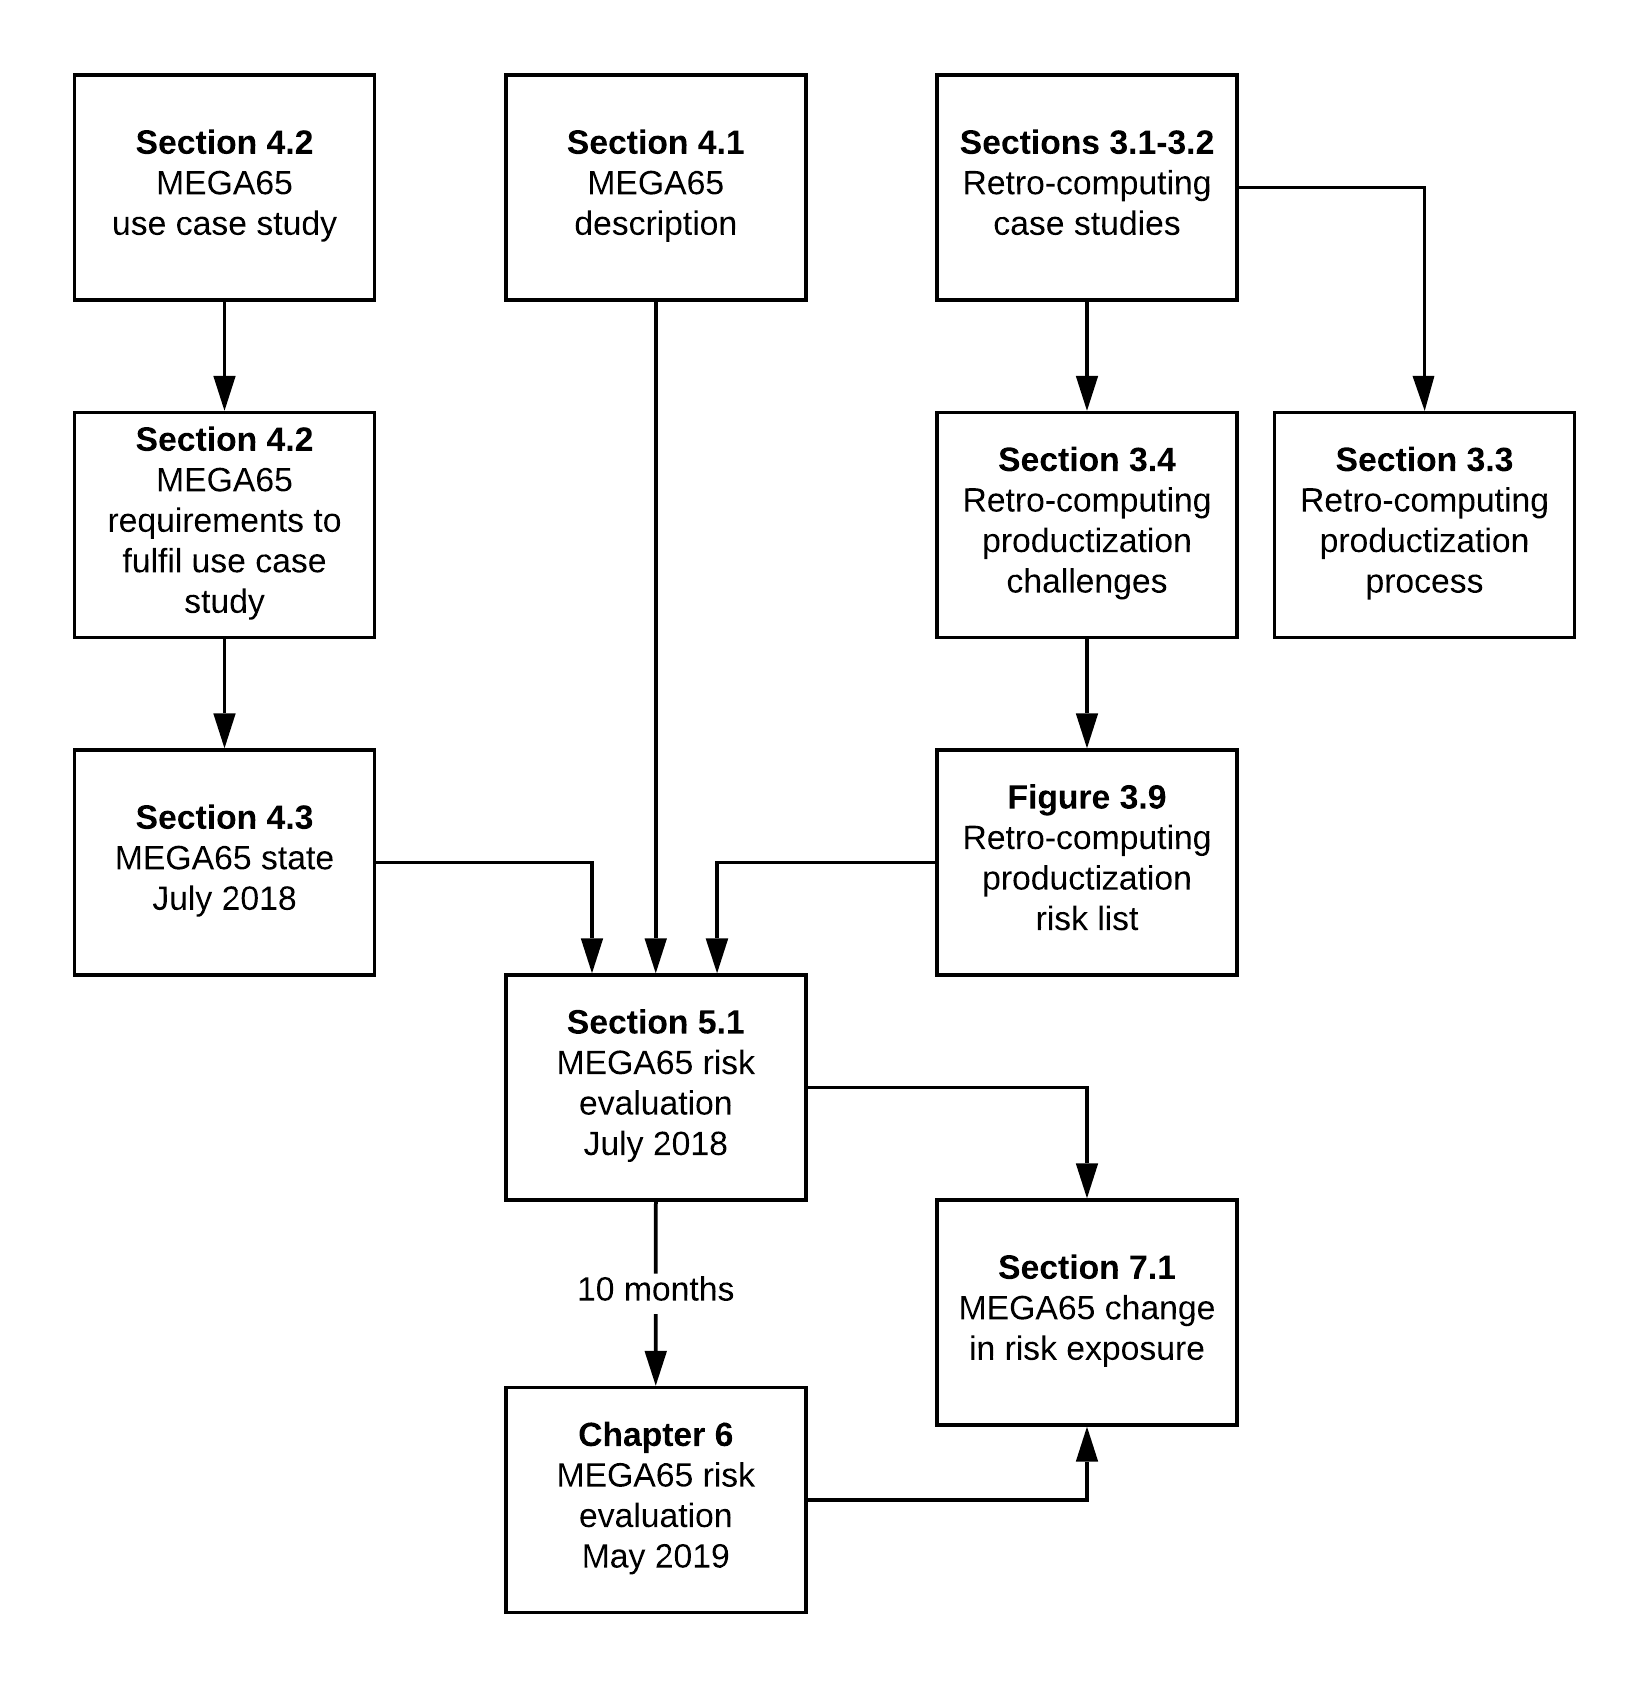
\includegraphics[width=.8\linewidth]{pics/thesis_methodology} 
\end{center} 
\caption{Flow diagram showing sections of this thesis and how they interact}
\label{methodology_diagram}
\end{figure}

%----------------------------------------------------------------------------------------
%----------------------------------------------------------------------------------------
\section{Contributions}
\label{contributions}
The contributions this thesis makes to retro-computing projects is categorised as follows:
\begin{enumerate}
\item Creates a body of knowledge exploring the retro-computing project productization process.
\item Creates a body of knowledge discussing the risks and challenges associated with retro-computing projects.
\item A risk evaluation of a specific retro-computing project, the MEGA65.
\item Practical, actionable recommendations to reduce the MEGA65 project's risk exposure.
\item Evidence of the benefit of those recommendations, gathered through a follow-up risk evaluation of the MEGA65 several months after providing the recommendations.
\end{enumerate}

%----------------------------------------------------------------------------------------
%----------------------------------------------------------------------------------------
\section{Structure of thesis}
Following this introductory chapter, a literature review in Chapter \ref{Chapter2} that focuses on the early home computing era, the growing complexity of computer hardware and software and its relationship to insecurity in modern computers. 

Chapter \ref{Chapter3} consists of case studies into several retro-computer projects with a focus on the process they followed and the challenges they faced in releasing a new product. After the case studies there is a discussion and synthesis of the productization process illuminated from the case studies. The challenges extracted from the case studies are then categorised into risks and these risks discussed and rated in terms of potential damage to retro-computing projects. 

Chapter \ref{Chapter4} is dedicated to explaining the MEGA65 project, its intended products and their state of development as of July 2018. This explanation takes the form of a description of the various aspects of the MEGA65 project, including the project's team characteristics, funding model and the products they are creating. Following the description of the MEGA65, there is a use case study conducted into the MEGA65 project's intended products, the MEGAphone and the desktop form-factor of the MEGA65, also called the MEGA65. 

A risk evaluation of the MEGA65 project in July 2018, provides the bulk of Chapter \ref{Chapter5}. Following the evaluation, the identified high-risk areas are discussed and advice is provided to the MEGA65 project on how to reduce their risk exposure. 

Finally, Chapter \ref{Chapter6} provides a second risk evaluation, taken 10 months after the first. The two risk evaluations are then compared and the changes in risk exposure are highlighted. A discussion of the results of the comparison and a conclusion follows, which ends the body of the thesis.
